\newpage
\section{Proposal for classification of optimization approaches}
\label{ch:Proposal}

% TODO:
% - Deriving:
%     - SAS Taxonomy by Krupitzer et al
%     - How did Krupitzer get to his taxonomy?
%     - 5W+1H questions
%     - Classification proposed by: The Application of ML
% - Proposing:
%     - Explain each part:
%         - Purpose
%         - Time
%         - Technique
%         - Location
%         - Concern
%     - What to explain:
%         - Why?
%         - How is it different from the other properties?

% \begin{itemize}
%     \item Deriving a classification for optimization approaches for Self-Adaptive Systems.
%     \item Proposing a classification for optimization approaches for Self-Adaptive Systems.
% \end{itemize}

% \paragraph*{Literature for this section:} \begin{itemize}
%     \item "The Application of Machine Learning in Self-Adaptive Systems: A Systematic Literature Review" \cite{ApplicationOfMachineLearning}
% \end{itemize}

% TODO: Deriving a classification}
% TODO: reference for MAPE
% TODO: FUSION and other OA just update a knowledge base (MAPE-K) and dont directly adapt the system
% so maybe RAC is not the perfect name for that category: changing structure vs providing knowledge
% approach: not if RAC is internal/external but if the OA is internal/external
% This would also make the classification more relevant!
Using the idea from Weyns et al. 2012 paper FORMS \cite*{FORMS} to compose Self-Adaptive Systems from
layers of base and reflective components, 
an Optimization Approach for Self-Adaptive Systems can be thought of
as a reflective component in a layer above the Self-Adaptive System.
This allows the application of multiple Optimization Approaches and even the 
optimization of Optimization Approaches.
It also establishes a connection between Optimization Approaches and Self-Adaptive Systems
and leads to the realization that a classification for Optimization Approaches of Self-Adaptive Systems
should be based upon the same principles as the classifications for Self-Adaptive Systems.
Another benefit is a clear distinction between Self-Adaptive Systems and Optimization Approaches for Self-Adaptive Systems:
While Self-Adaptive Systems and Optimization Approaches are both composed of reflective components and not base components,
the Self-Adaptive System adapts base components, while the Optimization Approach adapts other reflective components.
\newline
\par


Following Krupitzer's et al, 2015 \cite*{SurveyOnEngineeringApproaches} taxonomy for Self-Adaptive Systems,
a classification for Optimization Approaches of Self-Adaptive Systems should answer 
the 5W+1H questions by Salehie and Tahvildari, 2009 \cite*{LandscapeAndResearchChallenges}.
These questions are: Where, When, What, Why, Who and How?
% These questions are:
% \begin{itemize}
%     \item Where is the need for change?
%     \item When should a change occur?
%     \item What should be changed?
%     \item Why should something be changed?
%     \item Who should change something?
%     \item How should something be changed?
% \end{itemize}

\begin{figure}[h!]
    \centering
    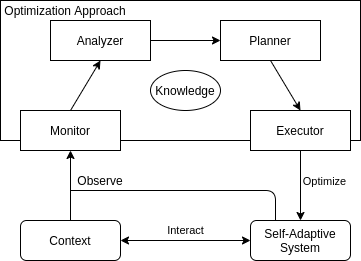
\includegraphics[width=0.6\columnwidth]{images/ClassificationProposal-OptimizationMAPEK.png}
    \caption{Mapping the optimization process to the MAPE-K feedback loop.}
    \label{fig:MappingOptMAPEK}
\end{figure}

Just like the adaptation process of Self-Adaptive Systems can be understood using
the MAPE-K (Monitor-Analyze-Plan-Execute with Knowledge) feedback loop by Kephart and Chess, 2003 \cite*{VisionOfAutonomicComputing}.
The process of optimizing a Self-Adaptive System can also be expressed using the MAPE-K feedback loop:
\begin{itemize}
    \item Firstly the optimization approach has to constantly monitor the Self-Adaptive System and its context.
    \item The data gathered from monitoring can then be analyzed to decided wether or not an optimization is necessary and what should be optimized.
    \item After deciding that something should be optimized, there needs to be a plan on how to optimize.
    \item Lastly the planned optimization can be executed.
    \item For all of this the optimization approach requires knowledge about the Self-Adaptive System and its context.
\end{itemize}

% TODO: Proposing a classification
% TODO: transition to proposal
\newpage
\begin{figure}
    \centering
    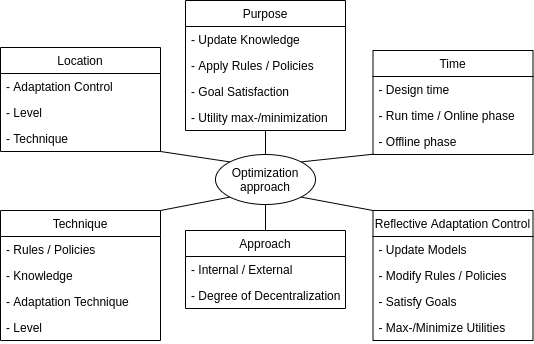
\includegraphics[width=0.8\columnwidth]{images/ClassificationProposal-WithDimensions.png}
    \caption{The proposed classification for Optimization Approaches for Self-Adaptive Systems}
    \label{fig:Proposal}
\end{figure}

\subparagraph*{Location}
Where in the system is an optimization necessary? \\
There are three main parts in a Self-Adaptive System that can require optimizations during its lifetime.
These are:
\begin{itemize}
    \item The Adaptation Control.
    \item The Level on which adaptations are performed
    \item The Technique that is used to perform adaptations.
\end{itemize}

\subparagraph*{Time}
When are optimizations performed? \\
Similarly to Self-Adaptive Systems, Optimization Approaches can be differentiated by comparing when they perform optimizations.
There are three different phases during the lifetime of a Self-Adaptive System where optimizations can occur.
These are:
\begin{itemize}
    \item At the runtime of the system, which can also be called the online phase.
    \item During the design time of the system.
    \item While training the system or during its offline phase.
\end{itemize}
The training phase can happen in parallel to the run and design time of the system.
Examples for this would be when the initial parameters for a Self-Adaptive System are chosen by training a domain model
or when generating a new model for the system by training an updated domain model parallel to the running system.

\subparagraph*{Technique}
What gets changed to perform the optimization? \\
What gets changed in a Self-Adaptive System relates to where an optimization is necessary.
Because of this, the following parts can be changed:
\begin{itemize}
    \item The Rules / Policies used by the Adaptation Decision Criteria.
    \item The Knowledge of the system, which for example can consist of domain models.
    \item The Adaptation Technique used by the Self-Adaptive System.
    \item The Level on which the Self-Adaptive System performs changes.
\end{itemize}
One could argue that the Goals or Utility functions of a Self-Adaptive System could also be changed to optimize its performance.
In most cases this is not advisable because Goals and Utility functions can encode information
like legal or safety parameters, of which the system has no intrinsic knowledge.

\subparagraph*{Purpose}
Why should an optimization occur? \\
This is perhaps the most important question for any Optimization Approach because it determines if an optimization is necessary.
There can be several reasons for performing an optimization in a Self-Adaptive System:
\begin{itemize}
    \item The system learned new information about for example its environment and needs to update its domain models.
    \item Because of external or internal changes, a Goal might not be satisfiable anymore.
    \item The difference of the actual versus the expected outcome of a rule / policy has exceeded a threshold.
    \item A Utility function needs to be maximized or minimized.
\end{itemize}

% TODO: Approach outside of Adaptation Control because of the original meaning
% of the question: level of automation vs human interaction.
% Self-Adaptive Systems: trivially should only be adapted by themselves.
% Optimization approaches: there might be human intervention necessary -> ML: learning trap, unpredicatability
\subparagraph*{Approach}
Who is responsible for performing the optimization? \\
\begin{itemize}
    \item Is there an internal component that performs changes or are they performed by an external actor.
    \item Which degree of decentralization is used?
    Is each component responsible for itself (fully decentralized), are all components optimized by a central entity (fully centralized)
    or is a hybrid approach used?
\end{itemize}

\subparagraph*{Reflective Adaptation Control}
How is the optimization applied to the system? \\
Just like the Self-Adaptive System can be described by its Adaptation Control,
which is responsible for applying changes to the system,
an optimization approach can also be described by how it applies its optimizations to the system.
In reference to FORMS by Weyns et al., 2012\cite*{FORMS}, which uses reflective operations to change
components in the system, the Adaptation Control of the optimization approach will be called Reflective Adaptation Control.

Unlike the Adaptation Control of Self-Adaptive Systems, 
the Reflective Adaptation Control does not have a dimension for the Approach, because it has its own separate dimension.
\begin{itemize}
    \item Adaptation Decision Criteria: \begin{itemize}
        \item Models: The system updates its models after receiving new information about its models.
        \item Rules / Policies: If the system detects, that it is in a state for which an adaptation rule/policy exists,
        it should perform that adaptation.
        \item Goals: Adaptation should be performed if the system does not meet pre-defined goals.
        \item Utility: An adaptation occurs to maximize or minimize a utility function.
    \end{itemize}
\end{itemize}

Because the proposed classification is based upon the MAPE-K feedback loop and the 5W+1H questions,
it is useful to map the classification to each of these models.
\begin{figure}[h!]
    \centering
    \begin{tabular}{|lcl|}
        \hline
        MAPE-K & & Optimization Approach \\
        \hline
        Monitor & & \\
        \hline
        Analyze & & Location\\
        \hline
        Plan & & Technique \\
        \hline
        Execute & & Reflective Adaptation Control \\
        \hline
    \end{tabular}
    \caption{How the MAPE-K feedback loop by Kephart and Chess, 2003\cite*{VisionOfAutonomicComputing}
    relates to the dimensions of the classification for Optimization Approaches for Self-Adaptive Systems.}
\end{figure}

\begin{figure}[h!]
    \centering
    \begin{tabular}{|lcl|}
        \hline
        5W+1H questions & & Optimization Approach \\
        \hline
        Where & & Location \\
        \hline
        When & & Time \\
        \hline
        What & & Technique \\
        \hline
        Why & & Purpose \\
        \hline
        Who & & Approach \\
        \hline
        How & & Reflective Adaptation Control \\
        \hline
    \end{tabular}
    \caption{How the 5W+1H questions by Salehie and Tahvildari, 2009 \cite*{LandscapeAndResearchChallenges}
    relate to the dimensions of the classification for Optimization Approaches for Self-Adaptive Systems.}
    \label{fig:5W1HProposal}
\end{figure}